\documentclass{standalone}

\usepackage{tikz}
\usepackage{pgfplots}
\usetikzlibrary{calc}
\pgfplotsset{compat=newest}

\begin{document}
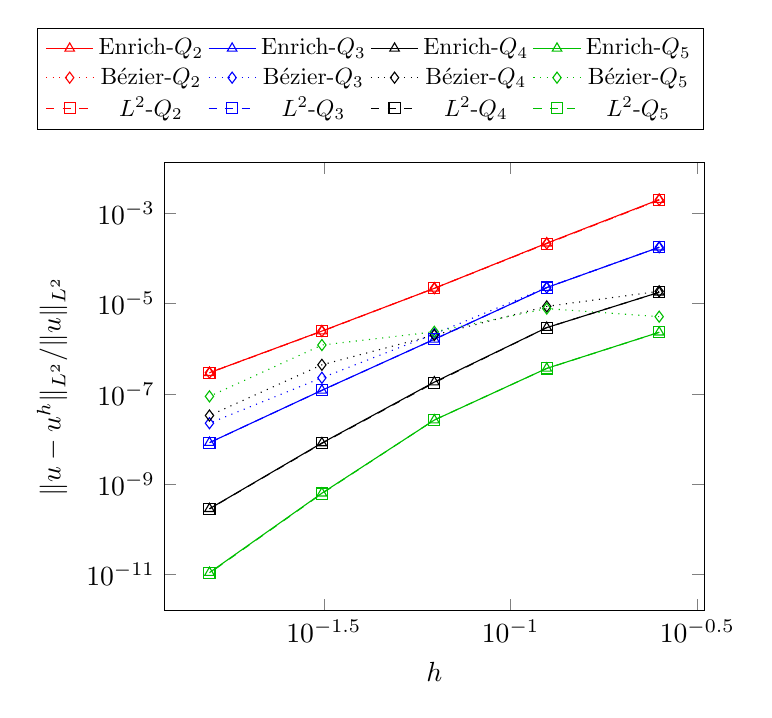
\begin{tikzpicture}
    \begin{loglogaxis}[
        legend columns=4,
    	legend style={at={(1,1.3)}, nodes={scale=.85, transform shape}},
        xlabel=$h$,
        ylabel=${\|u-u^{h}\|_{L^2}}/{\|u\|_{L^2}}$ 
    ]

    \addplot [color=red,mark=triangle] plot coordinates {

        (.25,       0.00201142)
        (.125,      0.000216982)
        (.0625,     2.17231e-05)
        (0.03125,   2.45455e-06)
        (0.015625,  2.94094e-07)
    };

    
    \addplot [color=blue,mark=triangle] plot coordinates {

        (.25,       0.000176233)
        (.125,      2.25779e-05)
        (.0625,     1.61513e-06)
        (0.03125,   1.19971e-07)
        (0.015625,  8.31133e-09)
    };

    \addplot [color=black,mark=triangle] plot coordinates {

        (.25,       1.77667e-05)
        (.125,      2.93108e-06)
        (.0625,     1.82319e-07)
        (0.03125,   8.16315e-09)
        (0.015625,  2.85295e-10)
    };

    \addplot [color=green!75!black,mark=triangle] plot coordinates {

        (.25,       2.31293e-06)
        (.125,      3.66743e-07)
        (.0625,     2.62891e-08)
        (0.03125,   6.30816e-10)
        (0.015625,  1.09866e-11)
    };

    
    \addplot [color=red,mark=diamond, every mark/.append style={solid}, dotted] plot coordinates {

        (.25,       0.00198141)
        (.125,      0.000214313)
        (.0625,     2.18727e-05)
        (0.03125,   2.45049e-06)
        (0.015625,  2.95754e-07)
    };

    
    \addplot [color=blue,mark=diamond, every mark/.append style={solid}, dotted] plot coordinates {

        (.25,       0.000176706)
        (.125,      2.26673e-05)
        (.0625,     2.11918e-06)
        (0.03125,   2.26883e-07)
        (0.015625,  2.23966e-08)
    };

    \addplot [color=black,mark=diamond, every mark/.append style={solid}, dotted] plot coordinates {

        (.25,       1.86969e-05)
        (.125,      8.65435e-06)
        (.0625,     2.00293e-06)
        (0.03125,   4.39797e-07)
        (0.015625,  3.31003e-08)
    };

    \addplot [color=green!75!black,mark=diamond, every mark/.append style={solid}, dotted] plot coordinates {

        (.25,       5.12909e-06)
        (.125,      7.73176e-06)
        (.0625,     2.36575e-06)
        (0.03125,   1.20514e-06)
        (0.015625,  8.79853e-08)
    };


    \addplot [color=red,mark=square, every mark/.append style={solid}, dashed] plot coordinates {

        (.25,       0.00196627)
        (.125,      0.000212527)
        (.0625,     2.17048e-05)
        (0.03125,   2.43161e-06)
        (0.015625,  2.92674e-07)
    };

    \addplot [color=blue,mark=square, every mark/.append style={solid}, dashed] plot coordinates {

        (.25,       0.000176052)
        (.125,      2.25899e-05)
        (.0625,     1.61489e-06)
        (0.03125,   1.19619e-07)
        (0.015625,  8.28756e-09)
    };

    \addplot [color=black,mark=square, every mark/.append style={solid}, dashed] plot coordinates {

        (.25,       1.77447e-05)
        (.125,      2.93245e-06)
        (.0625,     1.76997e-07)
        (0.03125,   8.00133e-09)
        (0.015625,  2.82775e-10)
    };

    \addplot [color=green!75!black,mark=square, every mark/.append style={solid}, dashed] plot coordinates {

        (.25,       2.3075e-06)
        (.125,      3.6553e-07)
        (.0625,     2.63764e-08)
        (0.03125,   6.19126e-10)
        (0.015625,  1.0707e-11)
    };

    \logLogSlopeTriangle{0.16}{0.075}{0.06}{5.9}{green!75!black};
    \logLogSlopeTriangle{0.16}{0.075}{0.205}{4.8}{black};
    \logLogSlopeTriangle{0.16}{0.075}{0.355}{3.9}{blue};
    \logLogSlopeTriangle{0.16}{0.075}{0.51}{3}{red};

    \legend{Enrich-$Q_2$\\Enrich-$Q_3$\\Enrich-$Q_4$\\Enrich-$Q_5$\\B\'ezier-$Q_2$\\B\'ezier-$Q_3$\\B\'ezier-$Q_4$\\B\'ezier-$Q_5$\\$L^2$-$Q_2$\\$L^2$-$Q_3$\\$L^2$-$Q_4$\\$L^2$-$Q_5$\\}
    \end{loglogaxis}
\end{tikzpicture}

\end{document}
